%%%
% Plantilla de Memoria
% Modificación de una plantilla de Latex de Nicolas Diaz para adaptarla 
% al castellano y a las necesidades de escribir informática y matemática%
% Editada por: Mario Román
%
% License:
% CC BY-NC-SA 3.0 (http://creativecommons.org/licenses/by-nc-sa/3.0/)
%%%

%%%%%%%%%%%%%%%%%%%%%%%%%%%%%%%%%%%%%%%%%
% Thin Sectioned Essay
% LaTeX Template
% Version 1.0 (3/8/13)
%
% This template has been downloaded from:
% http://www.LaTeXTemplates.com
%
% Original Author:
% Nicolas Diaz (nsdiaz@uc.cl) with extensive modifications by:
% Vel (vel@latextemplates.com)
%
% License:
% CC BY-NC-SA 3.0 (http://creativecommons.org/licenses/by-nc-sa/3.0/)
%
%%%%%%%%%%%%%%%%%%%%%%%%%%%%%%%%%%%%%%%%%

%----------------------------------------------------------------------------------------
%	PAQUETES Y CONFIGURACIÓN DEL DOCUMENTO
%----------------------------------------------------------------------------------------

%%% Configuración del papel.
% microtype: Tipografía.
% mathpazo: Usa la fuente Palatino.
\documentclass[a4paper, 20pt]{article}
\usepackage[a4paper,margin=1in]{geometry}
\usepackage[protrusion=true,expansion=true]{microtype}
\usepackage{mathpazo}
\usepackage{ stmaryrd }

% Indentación de párrafos para Palatino
\setlength{\parindent}{0pt}
  \parskip=8pt
\linespread{1.05} % Change line spacing here, Palatino benefits from a slight increase by default


%%% Castellano.
% noquoting: Permite uso de comillas no españolas.
% lcroman: Permite la enumeración con numerales romanos en minúscula.
% fontenc: Usa la fuente completa para que pueda copiarse correctamente del pdf.
\usepackage[spanish,es-noquoting,es-lcroman,es-tabla,,es-nodecimaldot]{babel}
\usepackage[utf8]{inputenc}
\usepackage{fontenc}
\selectlanguage{spanish}


%%% Gráficos
\usepackage{graphicx} % Required for including pictures
\usepackage{wrapfig} % Allows in-line images
\usepackage[usenames,dvipsnames]{color} % Coloring code
%\usepackage{subcaption}
\usepackage{subfig}
\graphicspath{{media/}}


%%% Matemáticas
\usepackage{amsmath}
\usepackage{physics} % para las derivadas parciales
\usepackage[Symbol]{upgreek} %pi

%%% Pseudocódigo

\usepackage[htt]{hyphenat}
\usepackage{algorithmicx}
\usepackage[ruled]{algorithm}
\usepackage{algpseudocode}

\newcommand{\alg}{\texttt{algorithmicx}}
\newcommand{\old}{\texttt{algorithmic}}
\newcommand{\euk}{Euclid}
\newcommand\ASTART{\bigskip\noindent\begin{minipage}[b]{0.5\linewidth}}
\newcommand\ACONTINUE{\end{minipage}\begin{minipage}[b]{0.5\linewidth}}
\newcommand\AENDSKIP{\end{minipage}\bigskip}
\newcommand\AEND{\end{minipage}}

%%% Código
\usepackage{listings}
\lstset{
  basicstyle=\ttfamily,
  columns=fullflexible,
  %frame=single,
  breaklines=true
}

%%% Tablas
\usepackage{tabularx}
\usepackage{float}
\usepackage{adjustbox}
\usepackage{booktabs}

% Enlaces y colores
\usepackage{hyperref}
\usepackage[dvipsnames]{xcolor}
\definecolor{webgreen}{rgb}{0,0.5,0}
\hypersetup{
  colorlinks=true,
  citecolor=RoyalBlue,
  urlcolor=RoyalBlue,
  linkcolor=RoyalBlue
}

%%% Bibliografía
\usepackage[backend=biber]{biblatex}
\addbibresource{citations.bib}


\usepackage{parcolumns}


\newcommand{\training}{\textit{training }}
\newcommand{\test}{\textit{test }}
\newcommand{\R}{\mathbb R}

%%% Subsubsection con letras
\renewcommand{\thesubsubsection}{\thesubsection.\alph{subsubsection}}

%%% Itemize, enumitem
\usepackage{paralist}
\usepackage{enumitem}
%----------------------------------------------------------------------------------------
%	TÍTULO
%----------------------------------------------------------------------------------------
% Configuraciones para el título.
% El título no debe editarse aquí.
\renewcommand{\maketitle}{
  \begin{flushright} % Right align
  
  {\LARGE\@title} % Increase the font size of the title
  
  \vspace{50pt} % Some vertical space between the title and author name
  
  {\large\@author} % Author name
  \\\@date % Date
  \vspace{40pt} % Some vertical space between the author block and abstract
  \end{flushright}
}

%% Título
\title{\textbf{Título}\\ % Title
Subtítulo} % Subtitle

\author{\textsc{Autor1,\\Autor2} % Author
\\{\textit{Universidad de Granada}}} % Institution

\date{\today} % Date

%-----------------------------------------------------------------------------------------
%	DOCUMENTO
%-----------------------------------------------------------------------------------------

\begin{document}

%-----------------------------------------------------------------------------------------
%	TITLE PAGE
%-----------------------------------------------------------------------------------------

\begin{titlepage} % Suppresses displaying the page number on the title page and the subsequent page counts as page 1
	
	\raggedleft % Right align the title page
	
	\rule{1pt}{\textheight} % Vertical line
	\hspace{0.05\textwidth} % Whitespace between the vertical line and title page text
	\parbox[b]{0.8\textwidth}{ % Paragraph box for holding the title page text, adjust the width to move the title page left or right on the page
		
		{\Huge\bfseries Práctica 3\\[0.5\baselineskip]\large Ajuste de datos usando modelos lineales\\[2\baselineskip]} % Title
		{\large\textit{\today}\\[0.5\baselineskip]Aprendizaje Automático\\[1.5\baselineskip] }% Subtitle or further description
		{\Large\textsc{Francisco Javier Sáez Maldonado}\\[0.5\baselineskip]fjaviersaezm@correo.ugr.es} % Author name, lower case for consistent small caps
		
		\vspace{0.4\textheight} % Whitespace between the title block and the publisher
		
		{\noindent \\[0.5\baselineskip] }\\[\baselineskip] % Publisher and logo
	}

\end{titlepage}

%% Resumen (Descomentar para usarlo)
%\renewcommand{\abstractname}{Resumen} % Uncomment to change the name of the abstract to something else
%\begin{abstract}
% Resumen aquí
%\end{abstract}

%% Palabras clave
%\hspace*{3,6mm}\textit{Keywords:} lorem , ipsum , dolor , sit amet , lectus % Keywords
%\vspace{30pt} % Some vertical space between the abstract and first section


%% Índice
{\parskip=2pt
  \tableofcontents
}
\pagebreak

\section*{Introducción}

En esta práctica, trataremos de realizar un estudio completo de un problema en el que se nos
presenta un conjunto de datos y nuestro objetivo es seleccionar el mejor predictor lineal para
este conjunto de datos dado. Concretamente, estudiaremos dos conjuntos de datos extraidos
de la web \href{https://archive.ics.uci.edu/ml/index.php}{UCI-Machine Learning Repository}.

Utilizaremos uno de ellos para tratar de ajustar un modelo lineal a un problema de regresión, y otro conjunto diferente de datos para ajustar otro modelo lineal a un problema de clasificación multiclase. El objetivo será realizar un estudio de los datos, evitando en todo momento el \emph{data snooping}, y argumentar si se utilizan ciertas técnicas de preprocesado de datos antes de escoger el modelo final.

Trataremos primero el problema de regresión y posteriormente el de clasificación.

\section{Regresión}

\subsection{Estudio del conjunto de datos. Identificación de $\mathcal X,\mathcal Y,f$.}

Lo primero que debemos hacer es realizar una buena comprensión de la información que tenemos sobre los datos para comprender un poco más nuestro problema.

Nuestro primer conjunto de datos, \cite{superdata}, contiene características de ciertos elementos superconductores. Junto con estas características, se nos presenta una \emph{temperatura crítica}, que en \cite{hamidieh} lo denominan $T_c$ siendo un problema similar al que vamos a abordar, obtenida para un superconductor que posea estas características. También se nos presenta un archivo en el que se nos dan las fórmulas químicas de los superconductores, pero este archivo no será relevante para nosotros.

Las características que obtenemos para este problema han sido generadas utilizando diferentes técnicas aplicadas a cada dato que se tenía inicialmente. Algunos de estos datos son su masa atómica, la energía requerida para ionizar el átomo, la densidad, la afinidad a nuevos electrones, temperatura de fusión, conductividad termal y la valencia del compuesto. Usando estos datos, se realizan una serie de transformaciones sobre estos valores para obtener el conjunto de datos final, limpiándolos durante el proceso de preparación, lo cual nos da unos datos con pocos errores o datos inútiles (se eliminan repetidos o aquellos que tengan $T_c = 0$).

Lo primero que nos encontramos acerca de nuestros datos es la siguiente tabla:
\begin{table}[h]
  \centering
  \begin{tabular}{|l|l|l|l|}
    \hline
    Características         & Multivariable & Número de instancias & $21263$ \\ \hline
    Tipo de características & Reales        & Número de atributos  & $81$    \\ \hline
    Tareas asociadas        & Regresión     & Valores perdidos     & $N\backslash A$   \\ \hline
  \end{tabular}
  \caption{Datos contenidos en el conjunto de datos Superconductivity.}
\end{table}


Esta información nos resulta muy útil, pues obtenemos podemos observar que tenemos $81$ atributos para cada una de las $21263$ instancias. De aquí podemos obtener que el tamaño del conjunto de datos es bastante amplio, por lo que tendremos un buen conjunto de entrenamiento. Las características que obtenemos son reales, es decir, $x_i \in \mathbb R^{81}$. Para completar, vemos que no tenemos valores perdidos, por lo que nos ahorraremos en este caso tener que establecer una técnica para reconstruir estos valores.

Con la información proporcionada podemos decir que:

\begin{enumerate}
\item Nuestro conjunto de datos de entrada será
  $$\mathcal X = \{ x_i \in \R^{81}, \text{ con } i = 1, \dots , 21263 \},$$
  que luego dividiremos en subconjuntos de entrenamiento y test.

\item Nuestro conjunto de etiquetas, puesto que no se nos indica ninguna restricción sobre las temperaturas, podemos asumir que es:
  $$
  \mathcal Y = \{ y_i \in \R, \text { con } i = 1,\dots,21263\}.
  $$

\item Por último, nuestra función $f : \mathcal X \to \mathcal Y$ que asigne a cada vector de características una temperatura crítica.
  
\end{enumerate}

Hay que anunciar que los siguientes gráficos de visualizado de datos se han realizado posteriormente a realizar la separación en conjuntos de \emph{train} y \emph{test} de nuestro conjunto de datos, para evitar en todo momento el \emph{data snooping}.\\

Dibujamos ahora un gráfico en el que mostramos el diagrama de caja de los posibles valores que toma la temperatura $T_c$:

\begin{figure}[H]
  \centering
  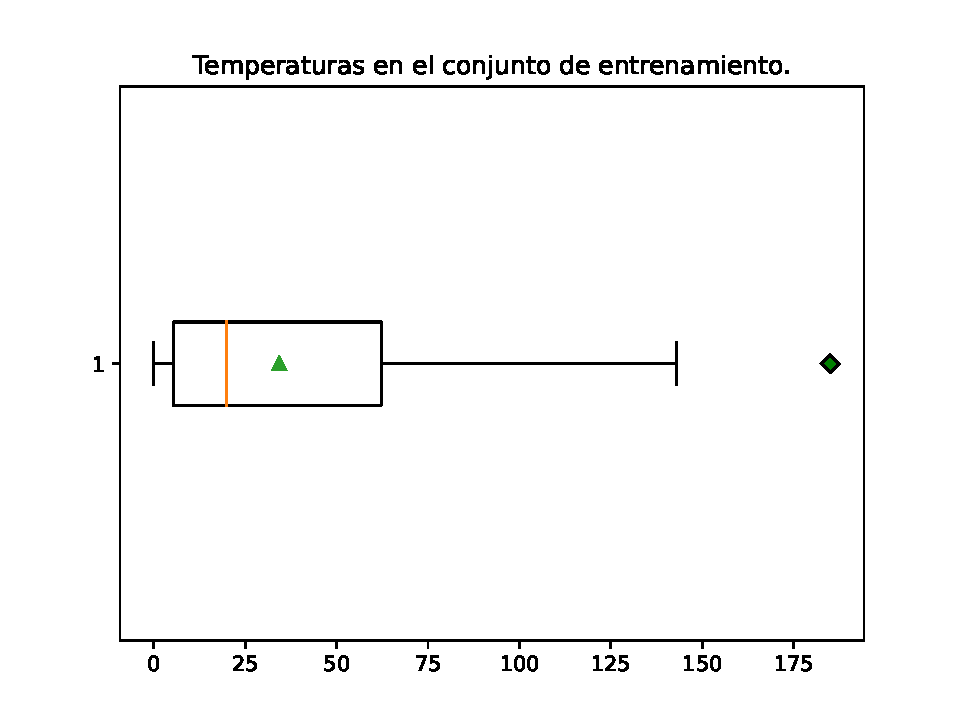
\includegraphics[scale = 0.4]{boxplot_y.pdf}
  \caption{Diagrama de caja de las temperaturas $T_c$ en el conjunto de entrenamiento.}
\end{figure}

Podemos ver que tenemos una variabilidad razonablemente amplia en los valores que toma $f$. Sin embargo, se observa que la mayoría de los valores de $f$ están concentrados en el intervalo $[0,50]$, pero también tenemos valores que se alejan bastante de este intervalo. Esto nos podría indicar que nuestra muestra está sesgada, en el sentido de que no tenemos muchos puntos $x_i$ en nuestro dataset que nos den valores altos de la temperatura $T_c$.  Como podemos ver, tenemos un dato que se aleja mucho de $1.5$ por el rango intercuartílico, que es lo que representan los \emph{bigotes} del diagrama de caja. Es por ello que podemos decir que este punto es posiblemente un \emph{outlier}.

Además, se ha tratado de encontrar si hay características que ofrezcan una desviación típica muy baja y que por ello pudieran no tener utilidad a la hora de entrenar nuestro modelo o hacer cálculos. Sin embargo, hemos encontrado que no hay ninguna característica con una desviación típica menor de $0.05$, por lo que no eliminamos por este criterio ninguna columna de nuestros datos.


\subsection{La clase de funciones $\mathcal H$. }

La clase de funciones a utilizar en este caso viene impuesta por el enunciado del ejercicio. En este caso, utilizaremos la clase de las funciones lineales:
$$
\mathcal H = \{ h(x) = w^T x \ : \ w \in \R^{n+1}\}.
$$

Tenemos que destacar que, aunque se podría plantear aplicar funciones no lineales a las características dadas (ejemplo $\phi :\R^d \to \R^{k}$ dada por $\phi(x) = (1,x_1,\cdots,x_n,x_1x_1,x_1x_2,\cdots,x_dx_d)$, no se hace en este caso pues estaríamos añadiendo ua complejidad a la clase de funciones sin saber realmente si esto sería útil de cara a la generalización o no. Es por ello que, al no tener en la información sobre los datos que se nos proporciona ningún motivo para hacerlo, se decide no aplicar ninguna transformación de este estilo a los datos.

Una vez fijada la clase de funciones, el modelo que usaremos para este problema es regresión lineal. No tiene sentido utilizar otros métodos como perceptron pues se usan en problemas de clasificación. 

Además, hay que comentar que para realizar esta regresión se utilizará el algoritmo de gradiente descendente estocástico (SGD), pues es bastante eficiente, unido a que podemos encontrar la implementación de esta regresión usando SGD en sklearn.

\subsection{Conjuntos de entrenamiento, validación y test.}

En este problema, tenemos un conjunto suficientemente grande de datos, que no viene previamente separado en subconjuntos de entrenamiento y test. En concreto, hemos mencionado ya que $N = 21263$ datos. Es por ello que se ha decidido usar un conjunto de entrenamiento con el $70\%$ de los datos, y dejar el $30\%$ para el conjunto de test. Para ello nos aprovechamos de la función \lstinline{train_test_split} de \lstinline{sklearn}.

Para elegir en nuestro conjunto de hipótesis antes de evaluar la función elegida en el conjunto de test, utilizaremos la conocida técnica \textbf{K-Fold Cross Validation}.

Esta técnica consiste en, si llamamos $X_{train}$ al conjunto de entrenamiento, realizar los siguientes pasos:
\begin{algorithm}[H]
  \caption{K-Fold Cross Validation}
  \begin{algorithmic}[1]
  \State $Vector\_Eouts = []$
  \For{i = 1,...,k}
    \State $ Datos_{val} \gets Particion_i$
    \State $ Datos_{train} \gets X_{train} \backslash Particion _i$
    \State $ Pesos \gets $ Entrenamiento en $Datos_{train}$
    \State $ Vector\_Eouts \gets Error(Pesos, Datos_{val})$

  \EndFor

  \State \textbf{return} Average $Vector\_Eouts$
  
  \end{algorithmic}
\end{algorithm}

Describiéndolo en pocas palabras, diríamos que partimos el conjunto de entrenamiento en $k$ subconjuntos y en cada iteración entrenamos nuestro modelo
con $k-1$ particiones y calculamos el error ``fuera de la muestra'' (lo llamamos así porque lo calculamos sobre el conjunto de datos de entrenamiento que \textbf{no} hemos usado para entrenar) usando la partición restante. Hacemos eso con todas las particiones y devolvemos una media de
los errores fuera de la muestra que hemos obtenido.

Obteniendo el error medio en validación usando este tipo de validación cruzada, podemos hacernos una idea de cómo de bueno (en media) será nuestro modelo fuera de la muestra. De hecho, sabemos que:

\textbf{Teorema.-} El error de validación cruzada $E_{cv}$ es un estimador insesgado de la esperanza del error fuera de la muestra en conjuntos de datos de tamaño $N-1$.

Usualmente, $K-$Fold cross validation se utiliza para estimar los parámetros con los que se entrenará nuestro modelo final, y una vez que se han estimado, se vuelve a entrenar el modelo usando
todos los datos de entrenamiento disponible para tener un modelo entrenado con un conjunto de datos lo mayor posible.


En nuestro caso, se usarán particiones \textbf{estratificadas} de los datos. Esto quiere decir que , dado un número de particiones (\emph{folds}) $k$, se divide el conjunto de entrenamiento en esas $k$ particiones con la salvedad de que se intenta mantener la distribución de datos existente en el conjunto en cada uno de los subconjuntos. En el caso de regresión, en cada partición obtenida tendremos valores de $f$ distribuidos como los tenemos en el conjunto de entrenamiento completo.

\subsection{Preprocesado de datos.}

Entramos en una de las fases más importantes de nuestro problema. Vamos a ver qué transformaciones haremos sobre nuestros datos antes de realizar la regresión.


En cuanto a los valores de nuestros datos, si tomamos una media de las desviaciones típicas $\sigma$ de los atributos de cada elemento de nuestro conjunto de datos, el resultado es:
\begin{lstlisting}[language = Python]
  Average Standard deviation of the features of the dataset per row: 1613.81306
\end{lstlisting}
Por lo que obtenemos que claramente los valores de los diferentes atributos no están en el mismo rango de escala. Es por ello que previamente al entrenamiento realizaremos una estandarización por atributos de nuestro conjunto de datos. Esto nos permitirá que sean comparables entre ellos.

Recordamos que tenemos 81 variables para cada dato. Nos interesa saber si todas estas variables son completamente útiles para el entrenamiento o nos interesa hacer una reducción de dimensionalidad en nuestro problema. Vamos a hacer una visualización las correlaciones entre las características para ver si algunas de ellas están altamente correladas.

\begin{figure}[H]
  \centering
  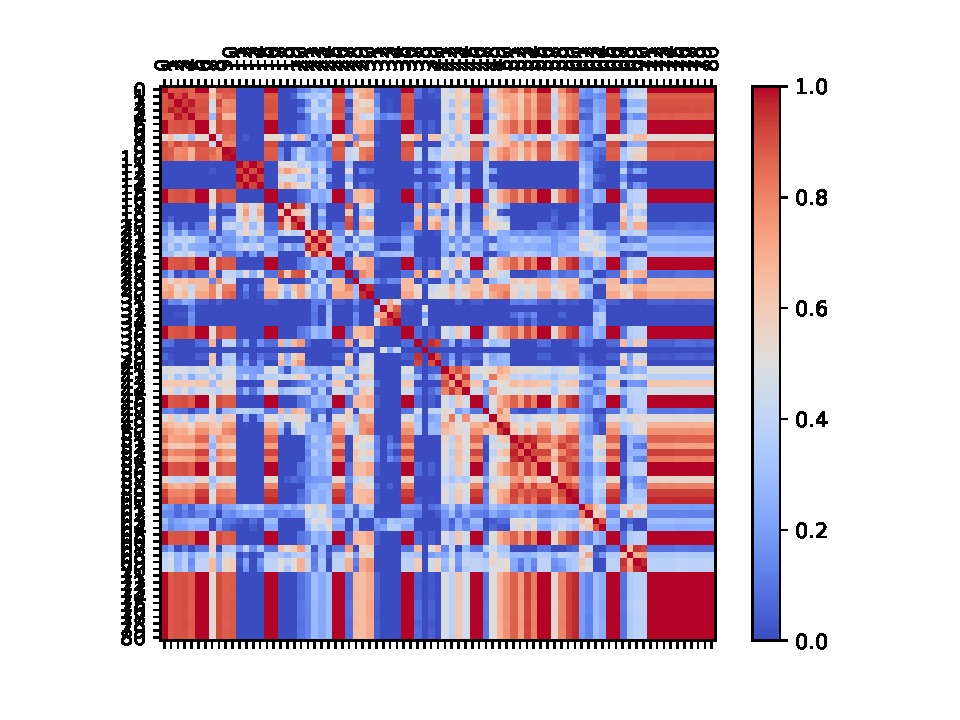
\includegraphics[width=0.55\linewidth]{media/corr-normalized.pdf}
  \caption{Matriz de correlaciones en el conjunto de entrenamiento estandardizado. }
  \label{fig:myfig:2}
\end{figure}

Como se puede observar a simple vista puede parecer que haya variables cuya correlación sea prácticamente igual a $1$, por lo que \textbf{puede darse el caso} de que sean suprimibles en el proceso de entrenamiento. En concreto, si nos quedamos con el triángulo superior y buscamos los valores mayores a $0.95$, obtenemos:
\begin{lstlisting}[language = Python]
  There are 23 variables which correlation with another is greater than 0.95
\end{lstlisting}
Por lo que hay 23 variables que podrían ser potencialmente eliminadas. 

La decisión sobre qué características son más relevantes para el entrenamiento, una vez mostrado empíricamente que hay variables altamente correladas, la vamos a hacer utilizando el \textbf{Análisis de componentes principales} (PCA).  Las \emph{componentes principales} de un conjunto de datos son una secuencia de vectores unitarios ortogonales entre sí y que marcan las direcciones que ajustan mejor a nuestro conjunto de datos, minimizando la distancia cuadrática media desde los puntos a la recta generada por cada vector. PCA es el proceso de encontrar estas componentes principales.

Una vez se han hallado, se reduce la dimensionalidad de nuestro conjunto de datos proyectando cada punto de datos a sus direcciones principales para obtener datos de menor dimensión, pero preservando la variabilidad de los datos lo máximo posible.

Se puede probar de hecho que las componentes principales son los vectores propios de la matriz de covarianzas de nuestro conjunto de datos, por lo que para hallarlas se debe hacer la descomposición de la matriz en valores singulares.

Tras aplicar el análisis de componentes principales, conseguimos que en nuestro conjunto de datos no haya correlaciones entre las variables. Esto nos ayuda además a reducir el \emph{overfitting} al tener menos variables dependientes. En nuestro caso, tras aplicar PCA haciendo que el algoritmo explique el $95\%$ de la varianza de nuestro conjunto de datos, obtenemos que nos quedamos con $17$ de las variables iniciales. Además, como podemos ver en la Figura \ref{fig:corr-pca}, las variables están completamente incorreladas.

\begin{figure}[H]
  \centering
  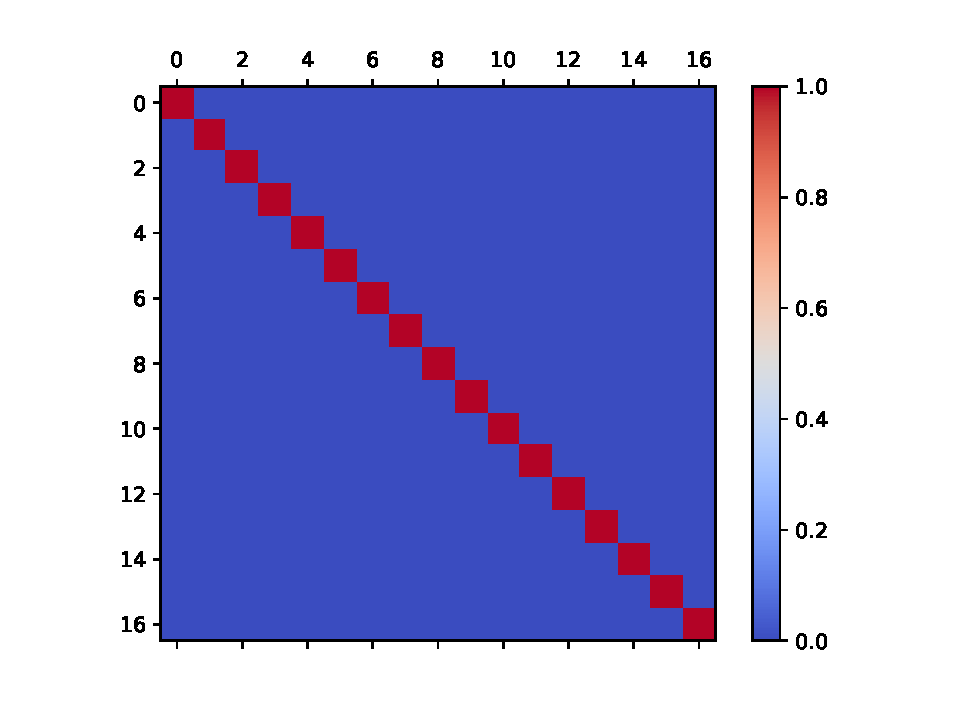
\includegraphics[width=0.55\linewidth]{media/corr-pca.pdf}
  \caption{Matriz de correlaciones tras aplicar PCA. }
  \label{fig:corr-pca}
\end{figure}


Sin embargo, quedarnos con tan pocas variables no nos asegura que el modelo entrenado con estas variables vaya ser mejor que el modelo entrenado con todas las variables.  Es por ello que cuando entrenemos, tomaremos para entrenar modelos con los datos reducidos en dimensionalidad y sin reducir.

Además, hay que comentar que se ha tratado de detectar \textbf{outliers} en nuestro conjunto usando \lstinline{IsolationForest} de \lstinline{sklearn}, pero el número de outliers encontrado era despreciable así que no se han eliminado del conjunto de entrenamiento.



\subsection{Métrica de error.}

En este problema, la métrica de error que utilizaremos es la estándar utilizada en problemas de regresión, el error cuadrático medio (MSE), que sabemos que viene dado por:
\[
MSE(h) = \frac{1}{N} \sum_{n = 1}^N (h(x_n) - y_n)^2.
\]
Donde sabemos que $N$ es el tamaño de la muestra usada e $y_j$ es el valor que toma la función $f$ en el punto $x_j$ para cada $j = 1,\dots ,N$. 

Esta métrica de error penaliza mucho los \emph{outliers} pues la distancia entre un punto lejano y el valor que predigamos mediante la regresión será grande, y error se incrementará en gran medida. En este caso sin embargo, no tenemos esos outliers. Hay que recordar además que no está acotada superiormente, por lo que podemos obtener valores muy grandes de error.

Sin embargo, esta métrica es idónea pues para que la regresión sea buena, lo que se pretenderá es que dentro de este conjunto de datos las distancias entre el valor predicho por nuestra regresión y el valor que tenemos como dato, $y_i$, sean lo más parecido posibles, por lo que es sin duda la mejor métrica de error a usar.

Hay que remarcar que para evaluar los modelos en el entrenamiento, este error se medirá en cada una de las particiones de la validación crucada y luego se hará una media de ellos para obtener:
$$
E_{cv} = \sum_{i = 1}^n MSE_i(h),
$$

que será el que se usará para determinar el modelo que escogeremos como el mejor finalmente.

Para medir el error final en el conjunto de test, usaremos también el coeficiente de determinación $R^2$. Este coeficiente mide la proporción de la varianza en la variable independiente que es predecible mediante la(s) variable(s) independiente(s). Concretamente, si consideramos $\bar{y}$ como el valor medio de las etiquetas, y consideramos las cantidades:
\[
SS_{tot} = \sum_i(y_i - \bar{y})^2 \quad y \quad SS_{res} = \sum_i(y_i - h(x_i))^2,
\]
calculamos $R^2$ como:
$$
R^2 =  1 - \frac{SS_{res}}{SS_{tot}}.
$$

Para interpretar esta medida, hay que saber que cuanto mejor sea el ajuste, menor es el cociente ,y más cercano es el valor de $R^2$ a $1$, por lo que lo ideal es que $R^2$ sea lo más grande posible.

\subsection{Regularización y parámetros del modelo.}

A la hora de entrenar, se demuestra tanto empírica como teóricamente que aplicar \textbf{regularización} mejora sustancialmente el resultado de los modelos. En la teoría, la regularización nos limita la clase de funciones a utilizar, reduciendo así la dimensión VC de la misma, y por tanto mejorando la cota del error fuera de la muestra que podemos dar. Además, en la práctica, la regularización previene a nuestro modelo de \emph{sobreajustar} la muestra.

Existen muchos tipos de regularización que se pueden aplicar a la hora de entrenar. Comentaremos dos de las más frecuentes y utilizadas habitualmente. 

\begin{itemize}
   

    \item La regularización \textbf{Lasso} o \textbf{L1}, que también añade un érmino de penalización a la función de pérdida, pero que en este caso suma el valor absoluto de los pesos:
    $$
    L_{reg}(w) = MSE(w) + \lambda \sum_{i = 0}^N \abs{w_i}.
    $$

    \item La regularización \textbf{Ridge} o \textbf{L2} suma una término cuadrático a modo de penalización a la función de pérdida. Este término es equivalente al cuadrado de la norma de los pesos.  La nueva función de pérdida queda como:
    $$
    L_{reg}(w) = MSE(w) + \lambda \norm{w}_2^2 .
    $$
    Como hemos visto en teoría, esto es idéntico a minimizar el error cuadrático medio sujeto a que $\sum_{j = 0}^p w_j^2 < c$ para cierto $c\in \R$. Así, estamos haciendo que los coeficientes sean más pequeños y reduciendo la complejidad del modelo.
\end{itemize}

En ambos casos, estamos añadiendo a la pérdida una penalización multiplicada por un parámetro $\lambda$. Si reducimos la constante de penalización $\lambda$, el término que nos queda es igual que el error cuadrático medio, por lo que lo interesante sera ajustar bien este parámetro para que la regularización afecte de manera positiva al entrenamiento.

La diferencia entre ambas es que en la regularización $L_1$ ayuda a seleccionar variables eliminando aquellas que tienen menos relevancia. La $L_2$ funciona mejor cuando se piensa que todas las variables son relevantes para la predicción. Además, el término que ésta introduce es diferenciable lo cual tiene ventajas computacionales. 

En este caso ya habíamos tratado de seleccionar las características que mejor explicasen la varianza del conjunto mediante PCA. Es por todo ello que elegimos usar la regularización $L_2$ en este problema. Como el número de parámetros a entrenar no es muy elevado, se ha decidido optar también por ampliar nuestras opciones en la búsqueda del mejor modelo y usar \textbf{también} esta regularización sobre el total de las características. 
% https://medium.com/analytics-vidhya/l1-vs-l2-regularization-which-is-better-d01068e6658c

\subsubsection{Parámetros de búsqueda.}

Quedaría por discutir los demás hiperparámetros con los que vamos a realizar nuestro entrenamiento. Estimar los mejores parámetros para un modelo es una tarea compleja. La mejor opción en la práctica es tomar para cada hiperparámetro un conjunto de valores que sepamos empíricamente que han dado buenos resultados en problemas similares y hacer una búsqueda haciendo combinaciones de esos valores de hiperparámetros para tratar de encontrar cuál es la combinación que mejor se ajusta a nuestro problema completo. Todo ello lo podemos realizar con la función de \lstinline{sklearn} :  \lstinline{GridSearchCV}.

Esta función, recibe como parámetros:
\begin{enumerate}
\item \lstinline{estimator} el estimador que va a utilizar para aproximar lo que nos interese. Podemos usar SVMs, Regresores Lineales, Perceptron... En nuestro caso, usaremos
  \begin{itemize}
  \item \lstinline{SGDRegressor} que nos realiza la regresión usando el descenso de gradiente estocástico.
  \item \lstinline{Ridge} que nos realiza la regresión usando la regularización $L2$.
  \end{itemize}
\item \lstinline{param_grid}, un diccionario que especifica para cada estimador que le demos el conjunto de hiperparámetros por los que tendrá que explorar. Explicaremos más adelante qué conjunto de parámetros a probar le pasaremos a la función.
\item \lstinline{scoring}, un string que indica cuál es la estrategia para evaluar el resultado de la validación cruzada. En nuestro caso, debemos especificar \lstinline{"neg_mean_squared_error"}, pues queremos obtener el modelo que \textbf{menor} error cuadrático medio obtenga, y \lstinline{GridSearchCV} siempre intentar \textbf{maximizar} la estrategia proporcionada.
\item \lstinline{n_jobs}, que indica cuántos procesos correr en paralelo. Elegimos la opción $-1$ para que se hagan todos los posibles y acelerar así el entrenamiento.

\item \lstinline{cv}, que determina el número de particiones que se hacen para la validación cruzada. En este caso, le indicamos que haga $5-$fold cross validation.


\end{enumerate}



Queda por concretar los valores concretos que se le dan a los parámetros que se le pasan en el diccionario \lstinline{param_grid}. En concreto, tenemos que comentar:

\begin{itemize}
\item El parámetro de regularización $\lambda$, que le hemos dado los valores $[0.1,0.01,0.001,0.0001,0.00001]$. Se han escogido estos valores pues se usan habitualmente en la literatura sobre los valores a escoger para el parámetro de regularización. Por ejemplo en \cite{2013applied}.

\item El número de iteraciones \lstinline{max_iter}, que se le han dado los valores $[5000,10000]$. En algunos casos, usando las $5000$ iteraciones se nos indica mediante un \emph{warning} que no se llega a converger, pero no es un problema porque tenemos el mismo modelo pero con $10000$ iteraciones.

  \item Para el parámetro \lstinline{learning_rate} usado en el regresor lineal con SGD, se utilizan también varias versiones de modificación del parámetro. En concreto, se usa \lstinline{constant}, para manterner el parámetro constante, \lstinline{adaptive} para que el parámetro aumente o disminuya según se vaya aumentando o disminuyendo el error obtenido, y \lstinline{optimal}, para tratar de obtener el óptimo descenso en cada iteración.

\end{itemize}


\subsection{Selección de hipótesis.}

Llegados a este punto, es el momento de explorar nuestro espacio de parámetros para encontrar el modelo que menor $E_{cv}$  tenga. Hay que mencionar que estos resultados se han obtenido utilizando el procesador de mi ordenador portátil: \emph{AMD Ryzen 7 4800h with radeon graphics × 16}.

Finalmente, se decide por aplicar los mismos modelos con los mismos parámetros de búsqueda en dos preprocesados de los datos diferentes, para comprobar si la aplicación de la reducción de la dimensionalidad en este problema nos ayuda o empeora nuestros resultados. Para ello, nos basta crear dos \lstinline{Pipeline}s de python y ejecutar nuestro \lstinline{GridScoreCV} dos veces.

\begin{minipage}{\textwidth}
  \begin{parcolumns}{2}
    \colchunk{\begin{lstlisting}[caption=Pipeline Standardization]{Name}

        preprocess = [
          ("standardize",StandardScaler())
        ]
        
    \end{lstlisting}}

    \colchunk{\begin{lstlisting}[caption=Pipeline PCA]{Name}

        preprocess_pca = [
          ("pre-standardize", StandardScaler()),
          ("PCA", PCA(n_components = 0.95)),
          ("standardize",StandardScaler())
        ]
    \end{lstlisting}}

    \colplacechunks
  \end{parcolumns}
\end{minipage}

Tras tener estos \emph{pipelines} creados y nuestro espacio de parámetros para la búsqueda creados, ejecutamos el método de búsqueda.

\begin{minipage}{\textwidth}
\begin{parcolumns}{2}
  \colchunk{\begin{lstlisting}[caption=Estandarizacion]{Name}
    
      Mejor en solo estandarizacion
      ----- Mejor regresor lineal encontrado ------
      - Parametros:
      Ridge(alpha=0.1, max_iter=5000)
      - Error en Cross Validation
      310.2545634883221
  \end{lstlisting}}

  \colchunk{\begin{lstlisting}[caption=PCA]{Name}

      Mejor usando PCA
      ----- Mejor regresor lineal encontrado ------
      - Parametros:
      Ridge(alpha=0.1, max_iter=5000)
      - Error en Cross Validation
      467.96851110824326
  \end{lstlisting}}

  \colplacechunks
\end{parcolumns}
\end{minipage}

Comparando los dos casos que hemos planteado para la búsqueda del mejor modelo, vemos que la hipótesis que mejor resultados nos ofrece en cuanto a minimización del $E_{cv}$, con una diferencia de más de $150$ unidades, es el modelo que \textbf{solamente realiza estandarización} en los datos y utiliza como regresor lineal el modelo \lstinline{Ridge} de \lstinline{sklearn}. Es por ello que nuestra hipótesis final $g$ será:
$$
g = \text{Ridge}(alpha = 0.1, max\_iter = 5000).
$$
Hay que destacar en los resultados que , cuando se utiliza preprocesamiento de los datos usando también PCA, el modelo que mejor resultados obtiene es el mismo. Esto nos puede indicar que, aunque estemos intentando mantener una gran cantidad de información explicada reduciendo las características, reducir las características nos está haciendo perder información sobre cómo se relacionan estas con la función $f$ que tenemos que aproximar.

La regresión usando \lstinline{Ridge} ha dado los mejores resultados aún variando un poco los parámetros. Se observa que para cualquier valor que se le proporcione de constante de regularización $\lambda$ (alpha según \lstinline{sklearn}), se obtienen errores en validación cruzada muy similares.

Además, se ha optado por usar este método de regresión porque es el que menor $E_{cv}$ nos da, pero usando el modelo de sklearn \lstinline{SGDRegressor} (que sabemos que hace regresión lineal usando SGD) con parámetros $\lambda = 0.0001$, $max\_iter = 5000$ y \emph{learning rate} adaptativo, se ha obtenido un $E_{cv} = 312.1983$, que se encuentra bastante cercano al error que nos da el mejor método.

Más información sobre los valores obtenidos para cada conjunto de parámetros fijo en cada uno de los algoritmos de minimización del error se puede observar en el apéndice \ref{apend:regresion} que se ha incluido para evitar rellenar el documento con tablas.

Mirando las tablas, podemos observar que en general el regresor que aplica la regularización de forma directa (\lstinline{Ridge}), ha obtenido resultados muchos mejores mientras que \lstinline{SGDRegressor} le ocurre que en algunos valores de $\lambda$ y formas de actualizar $\eta$, obtiene errores en cross validation demasiado grandes. Esto es posiblemente porque necesite un número de iteraciones muchísimo más alto para encontrar una recta de regresión que aproxime nuestros datos al nivel que lo hacen los demás aproximadores. Además, con algunos valores de estos mismos parámetros, el algoritmo no es capaz hacer qeu el error se aproxime al mínimo que sabemos que podemos obtener con otros parámetros.

\subsection{Error final fuera de la muestra.}

Nos queda por ver cómo de bien hemos conseguido \emph{``generalizar''} , usando el conjunto que hemos dejado desde el principio fuera de todas nuestras operaciones para evitar el \emph{data snooping}.



\begin{lstlisting}[language=Python]

  ------ RESULTADOS FINALES EN TEST -------

	- MSE: 313.4691035257312
	- R^2: 0.7366585080400442 

\end{lstlisting}



\newpage

\section{Clasificación}

\subsection{Estudio del conjunto de datos. Identificación de $\mathcal X, \mathcal Y, f$}

De nuevo, comenzamos observando la información que se nos proporciona del conjunto de datos. En este caso, nuestro nuevo conjunto de datos \cite{noauthor_uci_nodate} contiene características sobre impulsos eléctros que se han producido en motores. Estos motores tienen componentes intactos y componentes que están dañados. Las características se han medido en numerosas ocasiones mediante $12$ condiciones de trabajo diferentes, es decir: diferentes velocidades o cargas sobre el motor. Han sido medidas usandouna sonda de corriente y un osciloscopio.

Una vez medidas las características, se han generado más datos usando la descomposición EMD \cite{noauthor_hilberthuang_2021}, y se han calculado datos estadísticos como la media, desviación típica o la curtosis de las variables.

Una vez medidas las características, se determina una clase de motor a las que estas características pertenecen. Se ha dividido el conjunto en $11$ clases diferentes, que nosotros trataremos de separar utilizando modelos lineales. Veamos de nuevo una tabla con más información sobre los datos:


\begin{table}[h]
  \centering
  \begin{tabular}{|l|l|l|l|}
    \hline
    Características         & Multivariable & Número de instancias & $58509$ \\ \hline
    Tipo de características & Reales        & Número de atributos  & $49$    \\ \hline
    Tareas asociadas        & Clasificación     & Valores perdidos     & $N\backslash A$   \\ \hline
  \end{tabular}
  \caption{Datos contenidos en el conjunto de datos Sensorless Drive Diagnosis.}
\end{table}

Podemos comprobar que tenemos un número de instancias aún mayor que en el caso anterior y son de nuevo variables reales. Además, tampoco tenemos valores perdidos por lo que no tendremos que preocuparnos de tratar ese caso. 

Con esta información, podemos concluir que:

\begin{enumerate}
\item El conjunto de datos de entrenamiento serán vectores de $\R^{49}$ de características de un motor, por lo que podemos definirlo formalmente como:
$$
\mathcal X = \{ x_i \in \R^{49}, \text{ con } i= 1, \dots, 58509\},
$$
que dividiremos también en conjunto de entrenamiento y test.

\item Sabemos que los datos se han dividido en 11 clases. Además, estas clases se representan por un número del 1 al 11. Por tanto, el conjunto de llegada es:
$$
\mathcal Y = \left\{ y_i \in \{1,2,\dots,11\} \text{ con } i = 1,\dots, 58509\}\right\}
$$
\item El último elemento de nuestro problema es la función $f: \mathcal X \to \mathcal Y$, que nos dará para un vector de características de un motor una etiqueta según la clase a la que pertenezca.
\end{enumerate}


Tras separar el conjunto de test para evitar el data snooping, se ha tratado de representar gráficamente el conjunto de train con sus clases utilizando la conocida técnica \lstinline{t-SNE} (t-Distributed Stochastic Neighbor Encoding). Esta técnica requiere una serie de parámetros que dependen de la distribución de los datos y nos ayuda transformar el conjunto multidimensional en un conjunto con las componentes que nos interesen, que para visualización suelen ser $2$ ó $3$. 

%https://www.jmlr.org/papers/volume9/vandermaaten08a/vandermaaten08a.pdf

Sin embargo, es bien sabido que obtener los parámetros adecuados para que produzca los resultados deseados no es tarea sencilla. De hecho, en 

% https://distill.pub/2016/misread-tsne/

se muestra cómo dentro de una misma muestra, según los hiperparámetros que se usen en \lstinline{t-SNE}, se pueden dar diferentes proyecciones al plano euclídeo. 

Aún así, se ha intentado sin éxito probar diferentes combinaciones de parámetros (perplejidad, número de iteraciones,tasa de aprendizaje) para tratar de obtener algo de información sobre los datos, y el resultado es el siguiente:

\begin{figure}[H]
  \centering
  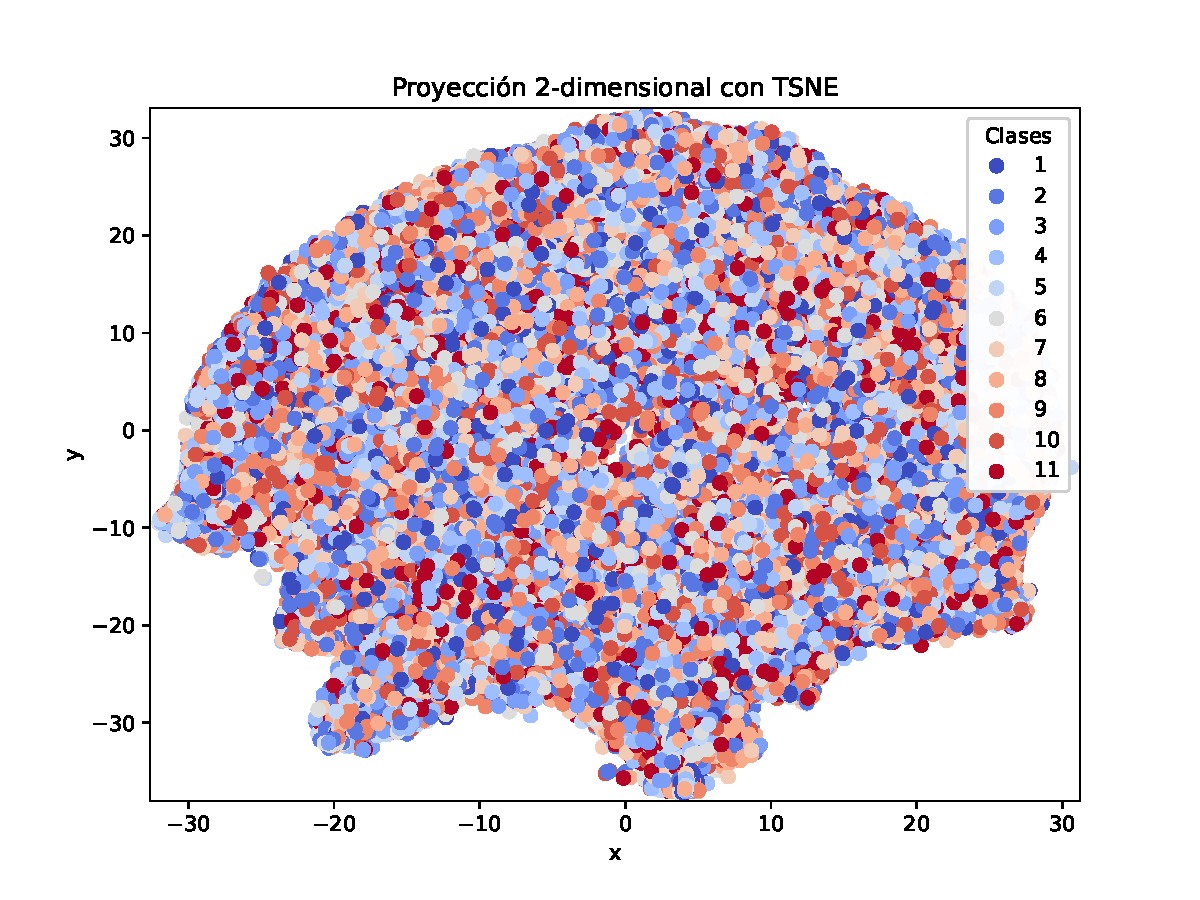
\includegraphics[width=0.55\linewidth]{media/tsne.pdf}
  \caption{Proyección al plano euclídeo y ajuste de \emph{t-SNE} con parámetros por defecto. }
  \label{fig:tsne}
\end{figure}

Se han usado los parámetros por defecto para el gráfico pues el resultado es muy similar al que ocurre si se utilizan parámetros más sofisticados.


%% Comentar la distribución en clases de los datos


\subsection{La clase de funciones $\mathcal H$.}


Ahora, las funciones deben ser del mismo tipo en el sentido de que en esencia deben ser lineales, es decir,
$$
h(x) = w^T x, \quad w \in \R^n
$$

Recordamos que cuando tratábamos de clasificar elementos en anteriores prácticas, como solo teníamos dos clases, nombrábamos una como positiva y la otra sería la negativa y podíamos tomar simplemente el signo de $h(x)$ como la etiqueta predicha para un elemento del conjunto. 

Ahora, estamos ante un problema de clasificación multietiqueta (en concreto, tenemos $11$) etiquetas, por lo que debemos emplear otra estrategia. En este caso , usaremos \emph{one-versus-all} (también conocida como \emph{one-versus-rest}). Debemos hacer un hiperplano $w_i$ para cada clase. 

Recordamos siguiendo lo que hemos visto en 
%% Referencia a learning from data
que como $w$ es ortogonal a todo vector que esté en el hiperplano, entonces podemos considerar a $h(x)$ una distancia con signo del punto $x$ al hiperplano salvo el cociente por $\norm{w}$. En \emph{one versus all}, consideramos que si queremos ver si un elemento $x \in \mathcal X$ pertenece a la clase $i-$ésima, se toma esta clase como la clase positiva y todas las demás como negativas, quedándonos así con un problema de clasificación binaria. Hacemos esto para todas las clases y, como $h_i(x) = w_i^T x$ es una distancia, consideraremos que la clase del elemento $x$ es la que obtenga el valor más grande. En el caso de no haber ninguno, se toma el valor más cercano a la frontera de clasificación. Matemáticamente, podemos expresar esto como:
$$
g(x) = \arg \max_i h_i(x).
$$

Es por ello que la clase de funciones que obtenemos en nuestro problema es la siguiente

$$
\mathcal H = \left\{ \ \arg \max_i w_i^T x  \ : \ w_i \in \R^n, i = 0,\dots,11\right\}.
$$

Igual que en el caso de regresión, no tenemos información suficiente para justificar la realización de transformaciones no lineales del espacio para obtener datos en el $\mathcal Z-$espacio que puedan darnos mejores resultados tanto dentro como fuera de la muestra, así que se decide no aplicar esas transformaciones.

\subsection{Conjuntos de entrenamiento, validación y test.}

En este caso, de nuevo tenemos todos los datos en un único fichero que tenemos que dividir nosotros. Optamos por volver a realizar una partición de $70\%$ para el conjunto de entrenamiento y $30\%$ para el conjunto de test.

También volveremos a utilizar en el entrenamiento $K-$\emph{Fold cross validation}, aunque en este caso es más relevante el hecho de que esta división sea estratificada, para mantener la distribución por clases de nuestro conjunto en cada una de las particiones y tener representantes de todas las clases en todos los subconjuntos y que estos no queden sesgados de cara al entrenamiento.

\subsection{Preprocesado de datos.}

\subsection{Métricas de error.}

En este caso debemos usar una métrica claramente diferente. Nos interesa un error que nos indique, dada una hipótesis $h$, cuántas veces de media obtenemos clasificaciones erróneas. Claramente, si $(x_n,y_n)$ representa un par: vector de atributos, etiqueta, entonces el error que queremos es:
$$
E(h) = \frac{1}{N} \sum_{i = 1}^N \llbracket h(x_n) \neq y_n \rrbracket.
$$

Como $\llbracket h(x_n) \neq y_n \rrbracket \in \{0,1\}$, tenemos que $E(h) \in [0,1]$ para toda hipótesis $h$. Esto se interpreta fácilmente porque podemos también considerar:
$$
Acc(h) = 1 - E(h),
$$
el acierto medio de la hipótesis.

\subsection{Regularización y parámetros del modelo.}

\subsection{Selección de hipótesis.}

\subsection{Error final fuera de la muestra.}



\newpage
\printbibliography

\newpage

\section{Apéndice}

\subsection{Resultados de los modelos en Regresión}
\label{apend:regresion}

Se incluyen las tablas con los resultados de los modelos para el problema de regresión. Se incluye una tabla con el preprocesado de solo estandarización y otra con estandarización y PCA.

\begin{table}[h!]
\begin{tabular}{lrlrr}
Regressor                        & $\lambda$ & $\eta$   & $max\_iter$ & $E_{cv}$                \\ \hline
SGDRegressor                     & 0.10000   & constant & 5000        & 636.93796          \\
                                 & 0.10000   & constant & 10000       & 636.93796          \\
                                 & 0.10000   & optimal  & 5000        & 2179664857.58336   \\
                                 & 0.10000   & optimal  & 10000       & 473348330.41042    \\
                                 & 0.10000   & adaptive & 5000        & 364.28276          \\
                                 & 0.10000   & adaptive & 10000       & 364.28276          \\
                                 & 0.01000   & constant & 5000        & 612.90878          \\
                                 & 0.01000   & constant & 10000       & 612.90878          \\
                                 & 0.01000   & optimal  & 5000        & 11859081963.44443  \\
                                 & 0.01000   & optimal  & 10000       & 2425006432.49777   \\
                                 & 0.01000   & adaptive & 5000        & 329.95897          \\
                                 & 0.01000   & adaptive & 10000       & 329.95897          \\
                                 & 0.00100   & constant & 5000        & 651.00770          \\
                                 & 0.00100   & constant & 10000       & 651.00770          \\
                                 & 0.00100   & optimal  & 5000        & 107610500809.15002 \\
                                 & 0.00100   & optimal  & 10000       & 22183869730.15907  \\
                                 & 0.00100   & adaptive & 5000        & 314.26437          \\
                                 & 0.00100   & adaptive & 10000       & 314.26437          \\
                                 & 0.00010   & constant & 5000        & 662.74988          \\
                                 & 0.00010   & constant & 10000       & 662.74988          \\
                                 & 0.00010   & optimal  & 5000        & 418399887304.88763 \\
                                 & 0.00010   & optimal  & 10000       & 418399887304.88763 \\
                                 & 0.00010   & adaptive & 5000        & 312.19840          \\
                                 & 0.00010   & adaptive & 10000       & 312.19840          \\
\textbf{Ridge}                            & \textbf{0.10000}   &          & \textbf{5000}        & \textbf{310.25456}          \\
                                 & 0.10000   &          & 10000       & 310.25456          \\
                                 & 0.01000   &          & 5000        & 310.25458          \\
                                 & 0.01000   &          & 10000       & 310.25458          \\
                                 & 0.00100   &          & 5000        & 310.25665          \\
                                 & 0.00100   &          & 10000       & 310.25665          \\
                                 & 0.00010   &          & 5000        & 310.25688          \\
                                 & 0.00010   &          & 10000       & 310.25688         
\end{tabular}
\caption{Resultados obtenidos según los parámetros usando sólo estandarización.}
\end{table}


\begin{table}[h!]
\begin{tabular}{lrlrr}
Regressor    & $\lambda$ & $\eta$   & $max\_iter$ & $E_{cv}$  \\ \hline
SGDRegressor & 0.10000   & constant & 5000        & 510.56864 \\
             & 0.10000   & constant & 10000       & 510.56864 \\
             & 0.10000   & optimal  & 5000        & 473.66396 \\
             & 0.10000   & optimal  & 10000       & 473.66396 \\
             & 0.10000   & adaptive & 5000        & 473.59663 \\
             & 0.10000   & adaptive & 10000       & 473.59663 \\
             & 0.01000   & constant & 5000        & 510.15916 \\
             & 0.01000   & constant & 10000       & 510.15916 \\
             & 0.01000   & optimal  & 5000        & 468.05363 \\
             & 0.01000   & optimal  & 10000       & 468.05363 \\
             & 0.01000   & adaptive & 5000        & 468.02466 \\
             & 0.01000   & adaptive & 10000       & 468.02466 \\
             & 0.00100   & constant & 5000        & 511.68573 \\
             & 0.00100   & constant & 10000       & 511.68573 \\
             & 0.00100   & optimal  & 5000        & 472.34160 \\
             & 0.00100   & optimal  & 10000       & 472.34160 \\
             & 0.00100   & adaptive & 5000        & 467.97220 \\
             & 0.00100   & adaptive & 10000       & 467.97220 \\
             & 0.00010   & constant & 5000        & 511.73210 \\
             & 0.00010   & constant & 10000       & 511.73210 \\
             & 0.00010   & optimal  & 5000        & 498.85089 \\
             & 0.00010   & optimal  & 10000       & 498.85089 \\
             & 0.00010   & adaptive & 5000        & 467.97353 \\
             & 0.00010   & adaptive & 10000       & 467.97353 \\
Ridge        & 0.10000   &          & 5000        & 467.96851 \\
             & 0.10000   &          & 10000       & 467.96851 \\
             & 0.01000   &          & 5000        & 467.96852 \\
             & 0.01000   &          & 10000       & 467.96852 \\
             & 0.00100   &          & 5000        & 467.96852 \\
             & 0.00100   &          & 10000       & 467.96852 \\
             & 0.00010   &          & 5000        & 467.96852 \\
             & 0.00010   &          & 10000       & 467.96852
\end{tabular}
\caption{Resultados obtenidos según los parámetros usando estandarización y PCA.}
\end{table}
\end{document}
